\section{Implementation and Analysis}
\label{SECIII}\label{sec:analysis}

\editorial{Should I mention \texttt{GStreamer} at all?} The detection method described above is much more efficient in terms of floating point operations than the traditional matched filter bank method.  However, time slices and conditional reconstruction greatly complicate queueing, synchronizing, and bookkeeping of intermediate signals.  A low latency implementation capable of recruiting more than one \textsc{cpu} core would be difficult to achieve within the familiar serial programming framework because of the nontrivial time-delay relationships between samples.  Due to these complications, we chose to prototype the search using an open source signal processing environment called \texttt{GStreamer}.  \editorial{Citation for \texttt{GStreamer}?}  Primarily used for playing, authoring, or streaming media on \texttt{Linux} systems, \texttt{GStreamer} is an integral component of the popular \texttt{Gnome} desktop.


\editorial{It would be good to illustrate the layout of this particular template bank: masses spanned, time slice layout \dots}
\editorial{Drew: I think this should say the FFT version of LLOID is almost 10 times faster than the conventional FFT method.}
\begin{table}[!h]
\caption{Operation counts per sample for six different detection methods.  The operation counts for \textsc{lloid} assume a reconstruction duty cycle of 5\%.  Note that the \textsc{fir} method with \textsc{lloid} is almost 10 times faster than the conventional \textsc{fft} method, despite having substantially lower latency.}
\begin{center}
\input{flop_budget}
\end{center}
\end{table}



\begin{comment}

% Ugly diagram!

\begin{figure*}[h!]
\begin{center}
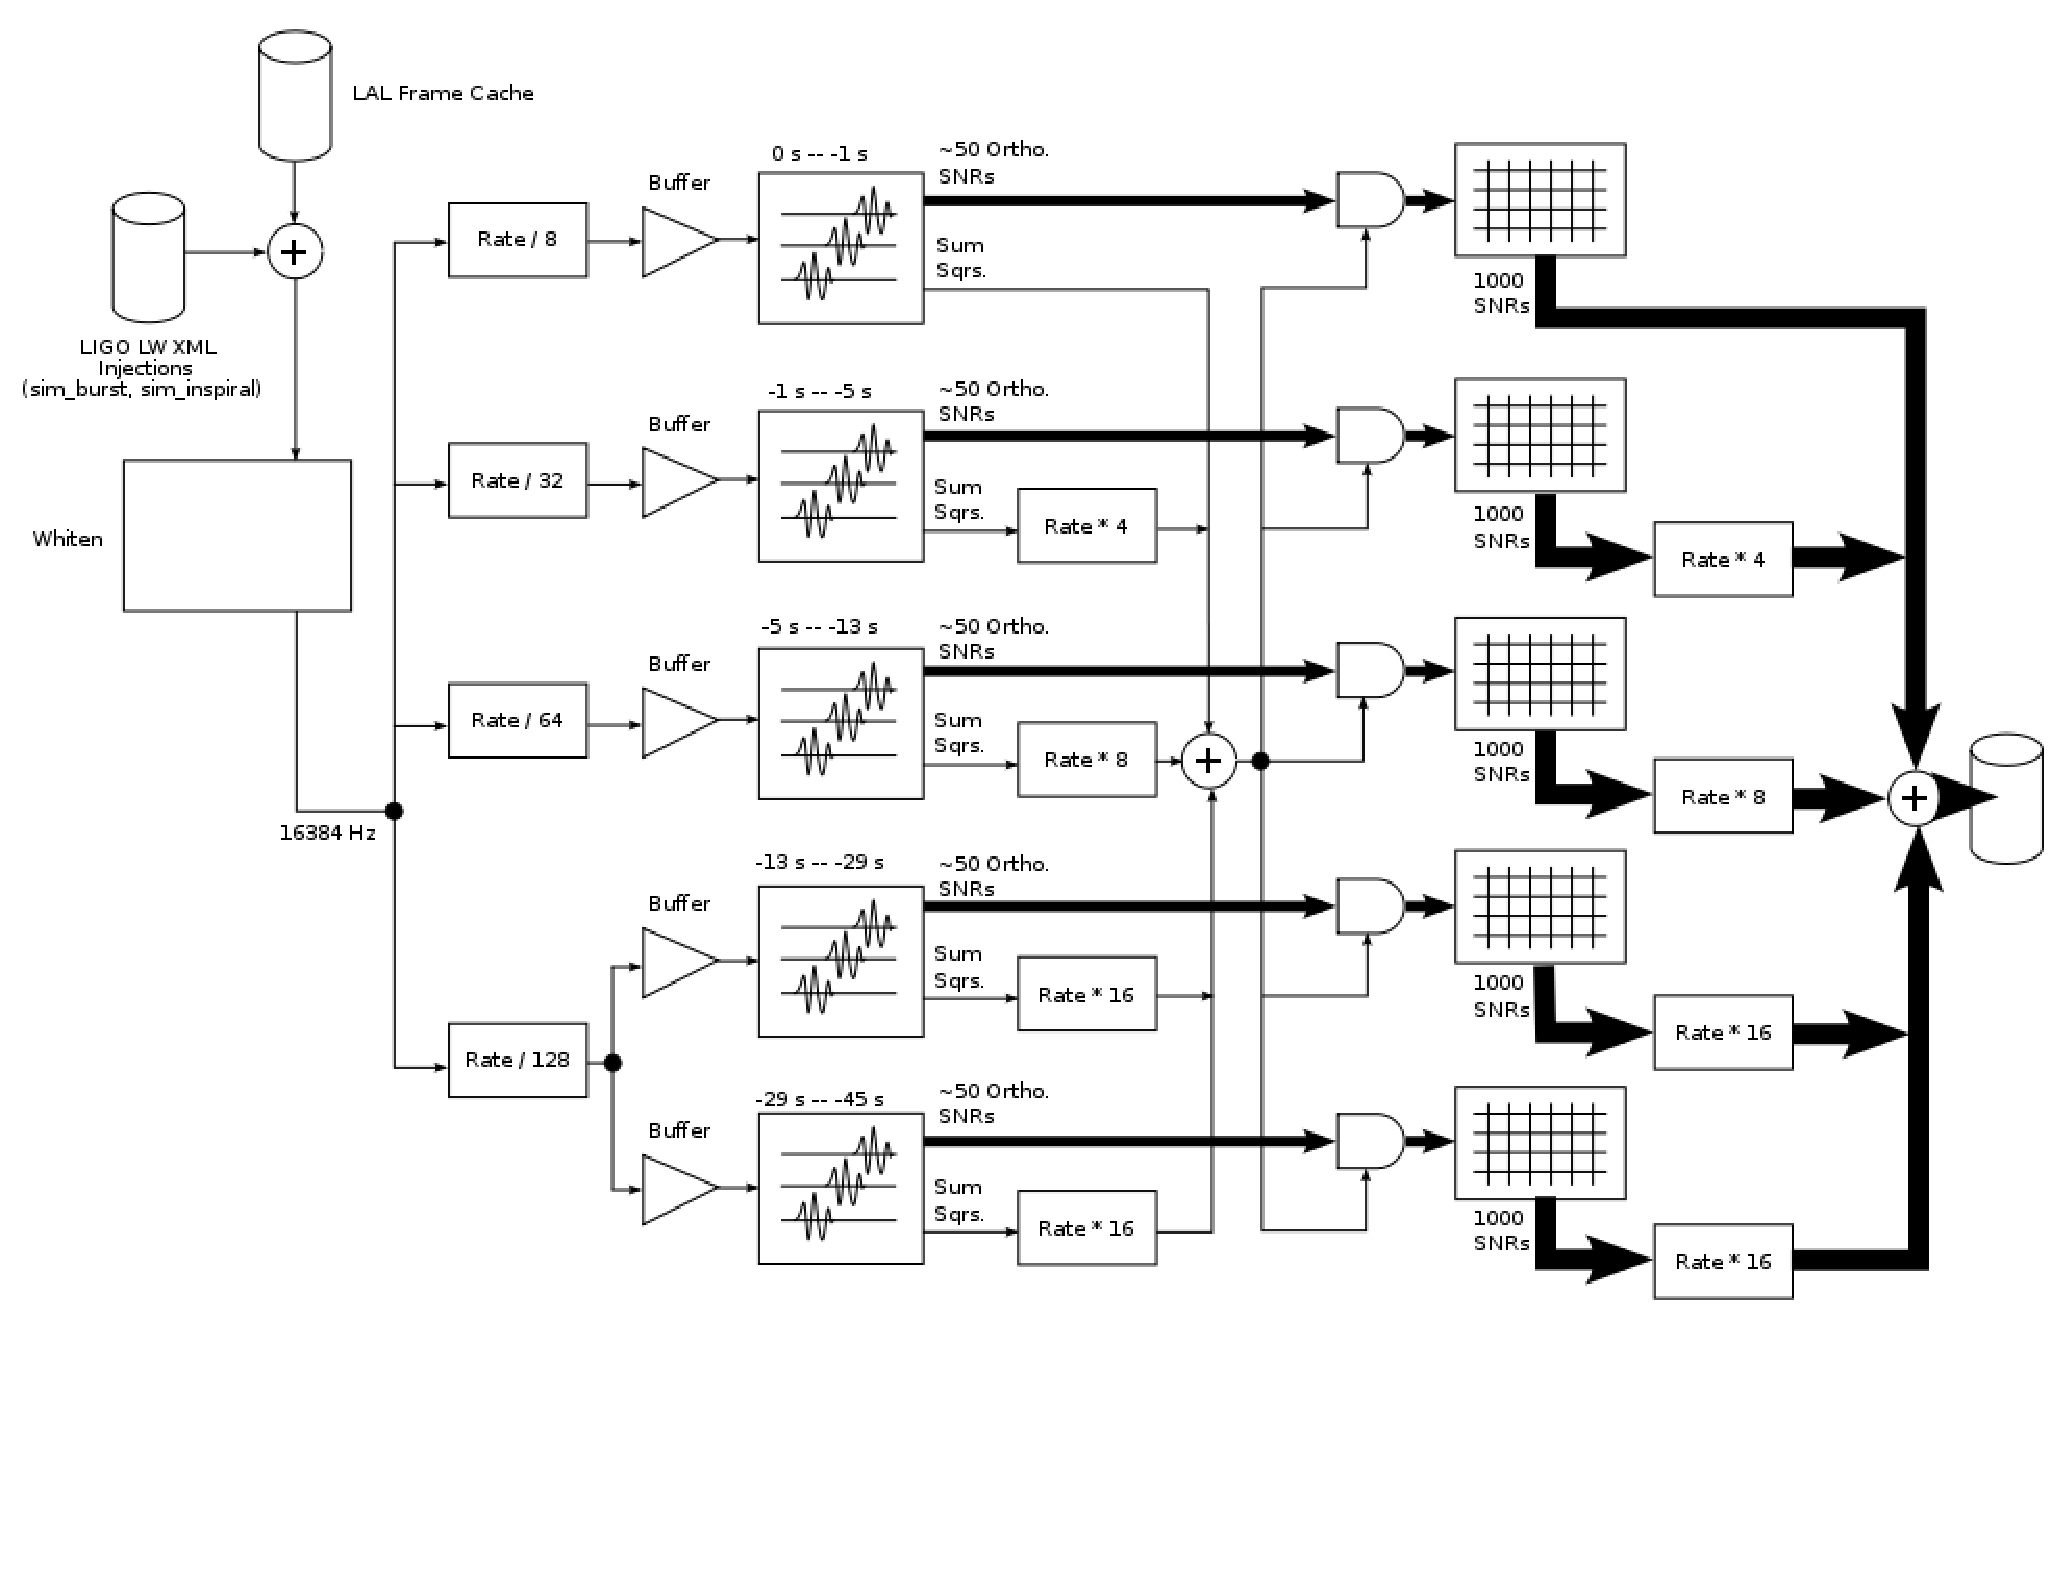
\includegraphics[width=1.0\textwidth]{figures/flow_chart.pdf}
\caption{\label{f:flowchart} 
}
\end{center}
\end{figure*}

\end{comment}
